\documentclass[usegeometry=true]{scrartcl}
\usepackage[ngerman]{babel}
\usepackage[T1]{fontenc}
\usepackage{lmodern}
\usepackage[utf8]{inputenc}
\usepackage{hyperref}
\usepackage{amssymb}
% Dimensionen bitte nicht ändern. 
\usepackage[left=2cm, right=2cm, top=2cm, bottom=2cm, bindingoffset=1cm, includeheadfoot]{geometry}
%Zeilenabstand bitte nicht ändern
\usepackage[onehalfspacing]{setspace}

\usepackage[backend=biber,style=numeric,]{biblatex}\addbibresource{literatur.bib}

\begin{document}

\subject{Projektbericht zum Modul Information Retrieval und Visualisierung Sommersemester 2022}
\title{Eine Analyse von Anzeigen auf einer deutschen
Gebrauchtwagenplattform aus dem Jahr 2023}
%\subtitle{Untertitel}% optional
\author{Johannes Göbel Matr.Nr.: }% obligatorisch
\date{\today}
\maketitle% verwendet die zuvor gemachte Angaben zur Gestaltung eines Titels
\vspace{10cm}
\begin{centering}

\hline
\vspace{0.5cm}
letzter commit: \\
Link zum Github Repository: \\
(\href{https://github.com/johannesgoebel/germany-used-cars-dataset}{https://github.com/johannesgoebel/germany-used-cars-dataset}) \\

Link zur Live Demo: \\
(\href{xxxx}{xxx})
    
\end{centering}
\pagenumbering{gobble}
% ----------------------------------------------------------------------------
\clearpage

\tableofcontents

\clearpage
% ----------------------------------------------------------------------------
% Gliederung und Text:
\pagenumbering{arabic}

\section{Einleitung}
Internetplattformen sind Digitalfirmen, die zwei oder mehr distinkte Nutzergruppen zusammenbringen. Sie werden zwischen B2B, bei denen zwei Geschäftskunden miteinander interagieren, und B2C, bei denen eine Seite durch einen Endkunden gebildet wird. In jedem Fall profitiert jede Seite durch eine Partizipation der gegenüberliegenden Seite am Netzwerk \cite{MUZELLEC2015139}. Dieser Effekt konnte bereits im späten 19.Jahundert bei der schleppend laufenden Adoption des Telefons beobachtet werden. Ein Telefon war nutzlos, wenn es niemanden gab, den man anrufen konnte. Das Netzwerk war erst wertvoll, als es viele Teilnehmer hatte – ein positiver direkter Netzwerkeffekt. \cite{evans2016matchmakers}
Internetmarktplattformen gewannen zuerst in den 1990er mit Firmen wie e-bay und Craiglist Bedeutung und fanden Anfang des Jahrtausends mit AirBnB, Booking.com und heutigen Entwicklungen wie Maschinensucher, wo ganze Industriemaschinen gehandelt werden können, einen steilen Aufstieg. Heute, 30 Jahre später, interagieren Menschen wie selbstverständlich mit solchen Plattformen. 
Selbst große E-Commerce Händler, wie Amazon, haben schon vor Jahren Marktplatzmechaniken in ihre Webseiten integriert. Diese Integration ist nahtlos, dass viele Nutzer gar nicht wissen, dass auf Amazon ein großer Preiskampf zwischen Drittanbietern ausgebrochen ist. (?????)
Gerade deshalb lohnt es sich einen Blick auf die Mechanismen von diesen Plattformen zu werfen und nachzuvollziehen, wie Verkäufer ihre Angebote bewerben.
Dies soll in dieser Arbeit am Beispiel von einer Gebrauchtwagenplattform geschehen. //
Dabei sollen in dieser Arbeit aber auch Markteffekte von PKWs mit unterschiedlichen Eigenschaften nicht außer Acht gelassen werden. Zu diesem Zweck werden die folgenden Forschungsfragen formulieren:

\begin{itemize}
    \item Wie hängt der Angebotspreis mit den angegebenen Merkmalen eines Gebrauchtwagens zusammen?
    \item Was sind die Werte für ein bestimmtes Fahrzeug? Wo befindet es sich im Vergleich zu den anderen Fahrzeugen? 
    \item Sind Preis- und Merkmalsunterschiede zwischen unterschiedlichen Automarken festzustellen, und wenn ja, wie?
\end{itemize}

\subsection{Anwendungshintergrund}
Zu diesem Zweck soll eine Webseite mit verschiedenen Visualisierungen erstellt werden, die es Nutzern ermöglicht schnell einen Überblick über die auf der Plattform vorhandenen Angebote zu erlangen und diese einzuordnen. \\
Die Daten hierzu sollen von einer echten Marktplattform programmatisch abgerufen werden um ein möglichst reales Bild einer solchen Plattform zu geben. Dies führt allerdings auch zu einem hohen Datenaufbereitungsaufwand.\\
\subsection{Zielgruppen}
Die Zielgruppe dieser Arbeit sollen Gebrauchtwagenverkäufer sein. \\
Die erste Zielgruppe zeichnet sich durch eine hohe Fachkenntnisse aus. Im Markt profitiert diese Gruppe von bestehenden Informationsasymmetrien, die sich durch Marktintransparenzen bilden. Durch Internetmarktplattformen sind diese Marktintransparenzen seltener zu finden. Beispielsweise können Käufer Preise vergleichen und können damit besser abschätzen, wie hoch der reale Marktpreis ist. \\
Daher interessieren professionelle Marktteilnehmer, wie auch trotz dieser technologischen Entwicklungen, eine relevante Marge erzielen können. 
Dieser Informationsbedürfnisse möchte diese Arbeit mithilfe von Visualisierungen zu Fahrzeugmerkmalen und Bewerbungsstilen decken. \\


\subsection{Überblick und Beiträge}
Die Daten werden hierzu in zwei unterschiedlichen Arten und Weisen aufgearbeitet. \\
Für die ersten beiden Visualisierungen – einen Scatterplot und einen Parallelplot – werden die beschafften Daten lediglich bereinigt und auf Ebene der einzelnen anzeigen betrachtet. 
Der Scatterplot soll es dem Nutzer hierbei ermöglichen Attribute miteinander gegenüberzustellen und der Parallelplot alle relevanten Merkmale überblicksartig einzusehen. \\
Für die dritte Visualisierung wurden die Daten auf Ebene der einzelnen Automarken betrachtet. Mittels eines Starplots soll dem Nutzer Aufschluss über Trends auf dieser Ebene gegeben werden. \\


\section{Daten}

\subsection{Datenverarbeitung}

Der Datensatz auf der Webseite Kaggle unter dem Titel "Germany Used Cars Dataset 2023" \href[]{https://www.kaggle.com/datasets/wspirat/germany-used-cars-dataset-2023}{Kaggle Datensatz}  bereitgestellt. Dieser umfasst über 200.000 Datensätze von der Gebrauchtwagenplattform Autoscout24 aus dem Jahr 2023, die durch Scraping gesammelt wurden.\\
In einem IPython Notebook wurden zunächst grundlegende Überlegungen angestellt, gefolgt von der Bereinigung des Datensatzes. Die Bewertung der Attribute erfolgte in Bezug darauf, ob sie für spätere Visualisierungen als (1) essenziell oder (2) sekundär betrachtet werden sollten. Fehlende Werte wurden entsprechend behandelt. Das Ziel der Bereinigung ist es in jedem Feld einen verarbeitbaren Wert vorfinden zu können.\\
Nach dem Löschen der unbenannten Indexspalte und der Zeilen ohne Werte in den Spalten "offer_description" oder "mileage_in_km", wurden fehlende Werte in der "color"-Spalte mit "unknown" aufgefüllt. Die "fuel_type"-Spalte wurde auf echte Antriebsarten überprüft, und unsinnige Daten in anderen Spalten wurden entfernt. Datensätze mit "power_ps" oder "power_kw" gleich null wurden gelöscht. \\

Die Spalte "fuel_consumption_g_km" wurde entfernt, da sie viele fehlende Werte enthielt und keine zusätzlichen Informationen gegenüber "fuel_consumption_l_100km" bot. Stringumwandlungen wurden für Elm in der "fuel_consumption_g_km"-Spalte und der "registration_date"-Spalte durchgeführt. \\

Dabei war ein Ziel die Vergleichbarkeit von Fahrzeugen unterschiedlicher Antriebsarten zu Gewährleisten, was beispielsweise bei den Daten zum Verbrauch ein Problem aufwarf. Wie sind die Daten von Pkws mit Verbrennungsmotor in l/100km und der Reichweitedaten für Elekoautos vergleichbar? Da diese nicht gewehrleistet werden konnte, 
- Erweiterung um Daten zu Anzeigetiteln (Zeichenlänge des Titels, Sentiment Analysis?, Anzahl Großbuchstaben) \\

Hier wurde der Datensatz auch um erste Merkmale wie offer_len, die die Anzahl der Buchstaben des Anzeigetextes widergibt, erweitert. \\

Im Anschluss daran wurde der Datensatz im CSV-Format exportiert und in Elm geladen. \\
Dabei wurden drei Datensätze exportiert: (1) "data.csv": Der Standarddatensatz, der rein wie oben beschreiben erstellt wurde. \\
(2) "avg_star_data.csv" und (3) "sum_star_data.csv": Die Datensätze für den Starplot, welche durch einen zusätzlichen Schritt erstellt wurden. Hier wurden die Daten der einzelnen PKWs nach Marken aggregiert bei (1) durchschnittswerte und bei (3) die summierten Werte.\\
Eine letzte Bemerkung soll zu einem größeren Problem beim Laden der Daten in Elm gewidmet sein. Leider traten bei der Erstellen der Daten mittels des iPython-Notebooks Probleme bei der Kodierung der Daten auf, so dass unsichtbare Characters in der CSV vorzufinden waren, welches dazu führte, dass Elm diese nicht ordnungsgemäß dekodieren konnte. \\

\subsection{Eignung der Daten}

In diesem Abschnitt wird diskutiert, inwieweit die vorliegenden Daten geeignet sind, die zuvor formulierten Forschungsfragen zu beantworten. \\

Grundsätzlich stammen die Daten aus dem Scraping einer Marktplatz-Webseite. Dies könnte ein realistisches Abbild des Marktplatzes liefern, sofern die Datenerhebung repräsentativ und stichprobenartig erfolgt ist. Es ist jedoch zu beachten, dass die Übertragbarkeit der Erkenntnisse aus der Datenanalyse und -visualisierung auf andere Plattformen möglicherweise eingeschränkt ist. \\

Zusätzlich ist anzumerken, dass keine Informationen darüber vorliegen, ob die vorliegenden Daten authentisch sind. Es ist unklar, ob die Daten ohne Vorauswahl oder Verfälschung durch das Scraping-Prozess gesammelt wurden. Andererseits gibt es derzeit keine erkennbaren Gründe, an der Authentizität der Daten zu zweifeln. \\

Eine letzte allgemeine Anmerkung ist, dass es sich bei der Beurteilung der Preise immer um Angebotspreise handelt. Es ist nicht bekannt, ob diese Fahrzeuge zu den genannten Preisen verkauft wurden oder nicht. Ebenfalls gehen natürlich weitere als die hier aufgeführten Merkmale in die Preisbildung ein. Beispielsweise ist es nicht klar, ob ein Auto eine Klimaanlage hat oder nicht, was die Preisvorstellung des Anbieters stark beeinflussen würde. \\

Die Daten enthalten Informationen über den Angebotspreis sowie verschiedene Merkmale von Gebrauchtwagen. Allerdings ist eine detaillierte Analyse der Beziehung zwischen diesen Merkmalen und dem Preis abhängig von der Qualität und Vollständigkeit der Daten. Einschränkungen könnten in fehlenden oder ungenauen Merkmalen liegen, die die Analyse beeinträchtigen könnten. \\

Die Datengrundlage um die Werte für ein einzelnes Fahrzeug und diese mit anderen zu vergleichen ist gegeben. Allerdings sind hier auch die allgemeinen Einschränkungen zu beachten. \\

Die Daten könnten eine Analyse der Preis- und Merkmalsunterschiede zwischen verschiedenen Automarken ermöglichen. Hierbei sind jedoch mögliche Einschränkungen zu berücksichtigen, wie ungleichmäßige Verteilung der Daten, so sind Einträge der Marke Audi viel häufiger im Datensatz vorhanden als Daten der Marke Proton. \\

Insgesamt sind die vorliegenden Daten geeignet, diese Forschungsfragen zu beantworten, vorausgesetzt, dass bestimmte Einschränkungen und Unklarheiten in der Datenqualität sorgfältig berücksichtigt werden. \\


\section{Visualisierungen}

\subsection{Analyse der Anwendungsaufgaben}

Analysieren sie die konkreten Anwendungsaufgaben, die die Lösung des Zielproblems durch die Anwender:innen bearbeitet werden müssen. 
Welche sinnvollen mentale Modelle helfen den Personen bei der Bearbeitung. 
%Welche Visualisierungen helfen den Personen, die die Software verwenden, sinnvolle mentale Modelle aufzubauen. 
Sind diese mentalen Modelle für sie notwendig, um die Aufgaben lösen zu können? Gehen sie bei ihrer Argumentation von den Anwendungsaufgaben aus und kommen sie dann zu den mentalen Modellen, deren Aufbau durch Visualisierungen unterstützt wird. 
\subsection{Anforderungen an die Visualisierungen}

Bei diesem Visualisierungsprojekt sind klare Anforderungen an die Darstellung von Daten von entscheidender Bedeutung. Um potenziellen Käufern eine hilfreiche Entscheidungsgrundlage zu bieten, sollten die Visualisierungen Aspekte wie Fahrzeugpreise, Kilometerstand, Baujahr, etc. einschließen. Eine intuitive Benutzeroberfläche ist unabdingbar, damit die Interessenten mühelos durch die Vielzahl von Angeboten navigieren können. Die Visualisierungen sollten daher die Möglichkeit bieten, Fahrzeuge anhand verschiedener Parameter zu filtern und zu vergleichen. Ein interaktiver Ansatz mit Filteroptionen und Hover-Funktionen könnte dabei helfen, detaillierte Informationen zu einzelnen Fahrzeugen abzurufen. Die visuelle Darstellung sollte sowohl informativ als auch ansprechend sein, um die Benutzererfahrung zu optimieren und eine effektive Entscheidungsfindung zu ermöglichen.  \\
Basierend auf diesen Metaanforderungen werden konkrete User Stories formuliert, die im Rahmen des Projektes addressiert werden sollen. \\
Funktionale User Stories: \\
\begin{enumerate}

    \item Als Nutzer möchte  Fahrzeuge anhand verschiedener Parameter wie Preis, Kilometerstand und Baujahr zu vergleichen, um schnell einen Überblick über die verfügbaren Optionen zu erhalten.
    
    \item Als Nutzer wünsche ich mir einen benutzerfreundlichen Parallelplot, der alle relevanten Informationen zu einzelnen Fahrzeugen auf einen Blick darstellt. Damit kann ich die Zusammenhänge zwischen den verschiedenen Parametern besser verstehen und gezielt nach meinen Präferenzen filtern.
    
    \item Als Nutzer interessiere ich mich für einen Star Plot, der mir eine visuelle Zusammenfassung der wichtigsten Merkmale verschiedener Fahrzeugmarken bietet. Dadurch kann ich schnell erkennen, wie sich die Marken in Bezug auf verschiedene Parameter unterscheiden.
\end{enumerate}
Nichtfunktionale User Stories: \\
\begin{enumerate}
    \item Als Anwender möchte ich eine ansprechende und intuitive Oberfläche erleben, die meine Navigation durch die Gebrauchtwagenanzeigen erleichtert. Die Visualisierungen sollten informativ und leicht verständlich sein, um mir eine effiziente Entscheidungsfindung zu ermöglichen.
    
    \item Als Nutzer erwarte ich, dass die Visualisierungen eine hohe Benutzerfreundlichkeit bieten, einschließlich interaktiver Elemente wie Filteroptionen und Hover-Funktionen. Dadurch kann ich gezielt nach meinen Anforderungen suchen und zusätzliche Details zu einzelnen Fahrzeugen abrufen.
    
    \item Als Anwender möchte ich die Möglichkeit haben, die Visualisierungen individuell anzupassen, indem ich verschiedene Parameter auswähle oder abwähle. Dadurch kann ich meine Suche und Analyse personalisieren und mich auf die für mich relevanten Informationen konzentrieren.
    
\end{enumerate}



\begin{figure}[h]
    \centering
    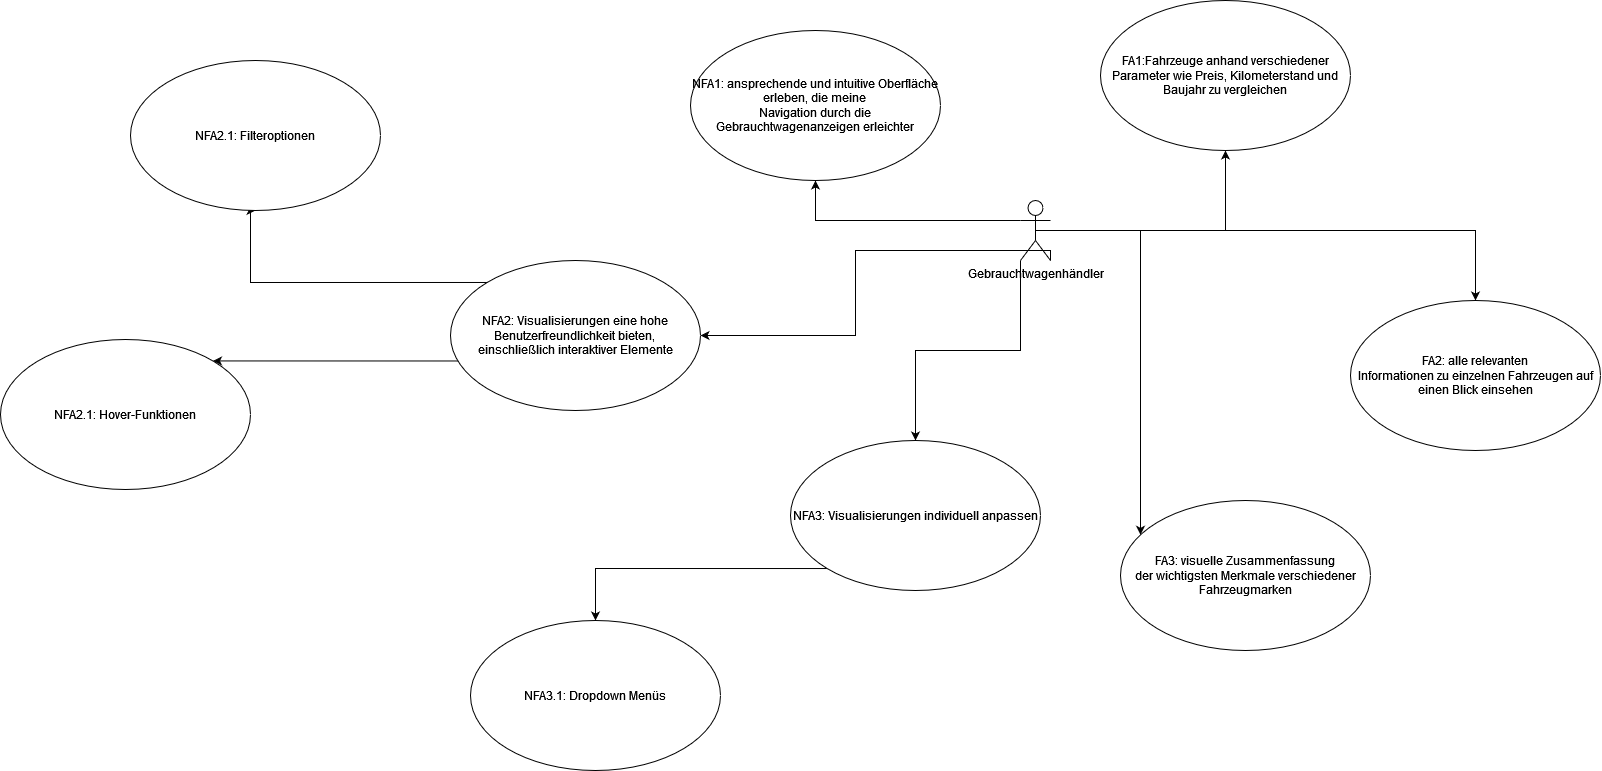
\includegraphics[width = \textwidth]{img/uc_diagram.png}
    \caption{Use Case Diagramm}
    \label{fig:uc_diagram}
\end{figure}

Aus diesen User Stories wurden dann funktionale und nicht funktionale Anforderungen in einem Use-Case Diagramm (Abbildung \ref*{fig:uc_diagram}) erstellt. \\
\subsection{Präsentation der Visualisierungen}
\subsubsection{Visualisierung Eins}

Der Scatterplot wurde entworfen, um Muster in den Gebrauchtwagenanzeigen aufzuzeigen und die Verteilung der Fahrzeuge in Bezug auf verschiedene Dimensionen sichtbar zu machen. Die Anpassung der X- und Y-Achsen kann über Dropdown-Menüs erfolgen, um eine direkte Vergleichsmöglichkeit von zwei Größen zu ermöglichen.\\

\begin{figure}[H]
    \centering
    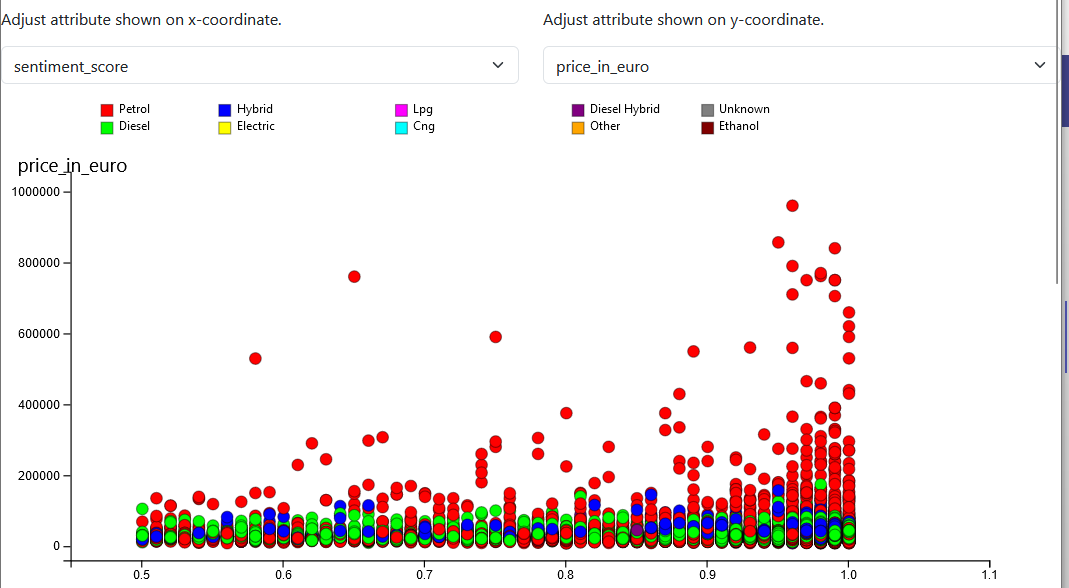
\includegraphics[width = \textwidth]{img/scatterplot.png}
    \caption{Scatterplot}
    \label{fig:scatter}
\end{figure}
\subsubsection{Visualisierung Zwei}

Im Parallelplot können mehrere Dimensionen gleichzeitig betrachtet werden, und die Linienverläufe zwischen den Achsen können auf mögliche Zusammenhänge hinweisen. \\
Die Anpassung der Achsen und Dimensionen im Parallelplot kann durch Auswahl der relevanten Attribute erfolgen. Dabei ermöglicht die visuelle Darstellung der Linienverläufe eine direkte Vergleichbarkeit verschiedener Fahrzeuge in Bezug auf diese Attribute. \\
Zusätzlich kann ein Datenpunkt mittels hovern eingefärbt werden. Dies erhöht die Bedienbarkeit. \\

\begin{figure}[H]
    \centering
    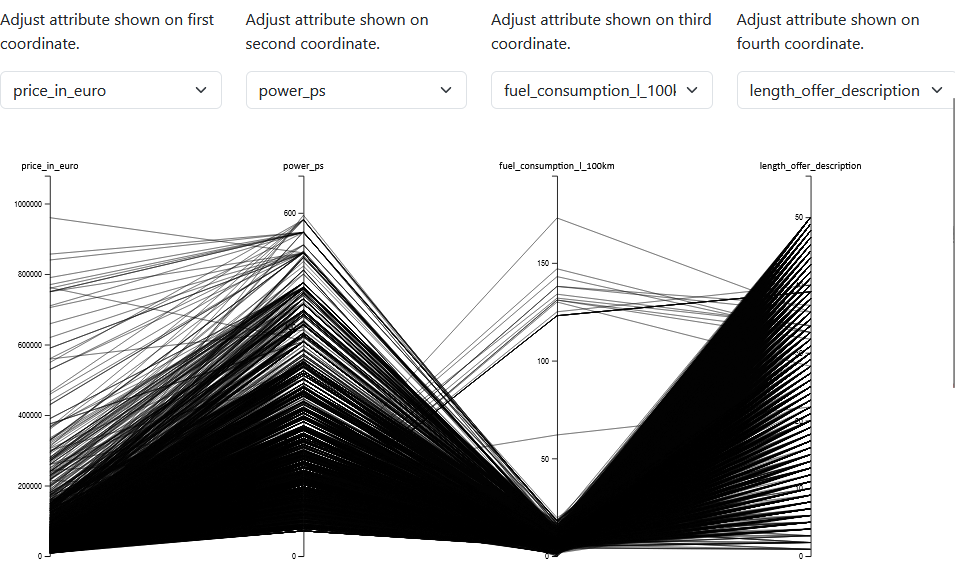
\includegraphics[width = \textwidth]{img/parallelplot.png}
    \caption{Parallelplot}
    \label{fig:scatter}
\end{figure}


\subsubsection{Visualisierung Drei}

Der Starplot bietet eine umfassende Visualisierung aller Attribute von Automobilanzeigen einer bestimmten Marke auf der Plattform. Durch diese Darstellung lassen sich alle relevanten Merkmale gleichzeitig betrachten und erleichtern somit einen schnellen Überblick. \\
Die Achsen des Starplots repräsentieren die verschiedenen Attribute, auf denen die durchschnittliche / summierte Attributsausprägung aller Anzeigen von Autos dieser Marke dargestellt ist. Dies ermöglicht einen schnellen Überblick über die Attributen dieser Marke. \\
Um den Starplot zu verwenden, wählen Sie die gewünschte Automarke aus, und der Plot wird automatisch generiert. Die Positionen der Linien auf den Achsen vermitteln Informationen über die relativen Werte der Attribute für jedes Fahrzeug. \\
Insgesamt ermöglicht der Starplot eine effektive und schnelle visuelle Analyse der Attribute aller Fahrzeuge einer ausgewählten Marke auf der Plattform. \\

\begin{figure}[H]
    \centering
    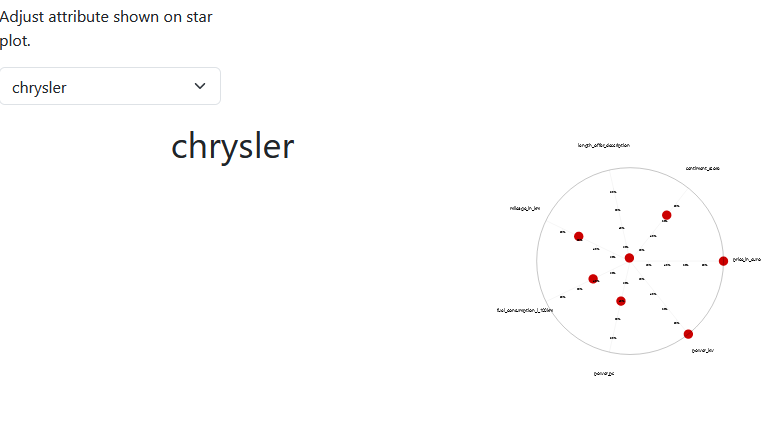
\includegraphics[width = \textwidth]{img/starplot.png}
    \caption{Starplot}
    \label{fig:scatter}
\end{figure}


\subsection{Interaktion}


Die Interaktion mit den Visualisierungen ist ein zentraler Aspekt des Projekts. Ein übergeordnetes Ziel besteht darin, alle Visualisierungen auf einer Seite anzuordnen, sodass ein einfaches Scrollen zwischen ihnen einen schnellen Gesamtüberblick ermöglicht. Um die Benutzererfahrung zu verbessern und die Visualisierungen an die Bedürfnisse des Nutzers anzupassen, sind verschiedene Anpassungsmöglichkeiten implementiert. \\

Insbesondere bieten das Scatterplot und das Parallelplot die Möglichkeit zur Anpassung durch einen Schieberegler (siehe Abbildung \ref{fig:schieber}). Durch Auswahl einer Jahreszahl werden in beiden Grafiken nur Daten aus diesem Jahr angezeigt. Diese Anpassung ist nicht nur benutzerfreundlich, sondern dient auch der Optimierung, da die Visualisierung aller Daten auf einmal zu langen Wartezeiten führen könnte. \\

Zusätzlich ermöglicht das Scatterplot eine weitere Anpassung durch zwei Drop-Down-Menüs. Diese Menüs dienen der Auswahl der Daten für die x- und y-Achse. Die Interaktion mit dem Scatterplot umfasst auch vier Dropdowns, jeweils für jede Achse. Durch diese Interaktion werden nicht alle verfügbaren Daten angezeigt, sondern nur die vom Nutzer gewünschten Werte. Dies trägt zur verbesserten Übersichtlichkeit und damit zur Nutzbarkeit für die Zielgruppe bei. \\
\begin{figure}[H]
    \centering
    
\includegraphics{img/interaktion1.png}
    \caption{Schieberegler}
    \label{fig:schieber}
\end{figure}

Die Auswahl der Daten im Parallelplot ist ähnlich möglich. Hier hat der Nutzer über vier Drop-Downs die gewünschten Daten einzubinden. \\
Auch im Starplot kann der Nutzer einen Datensatz - eine Marke - auswählen, die er/sie sich genauer anschauen will. \\


\section{Implementierung}

Beschreiben Sie die Implementierung ihrer Visualisierungsanwendung in Elm. Stellen die Gliederung ihres Quellcodes vor. Haben Sie verschiedene Elm-Module erstellt. Was war aufwändig umzusetzen, was ließ sich mit dem vorhanden Code aus den Übungen relativ einfach umsetzen? 

Wie sieht die Elm-Datenstruktur für das Model aus, in dem die verschiedenen Zustände der Interaktion gespeichert werden können.


\section{Anwendungsfälle}
Präsentieren sie für jede der drei Visualisierungen einen sinnvollen Anwendungsfall in dem ein bestimmter Fakt, ein Muster oder die Abwesenheit eines Musters visuell festgestellt wird. Begründen sie warum dieser Anwendungsfall wichtig für die Zielgruppe der Anwenderinnen ist. Diskutieren sie weiterhin, ob die oben beschriebene Information auch mit anderen Visualisierungstechniken hätte gefunden werden können. Falls dies möglich wäre, vergleichen sie die den Aufwand und die Schwierigkeiten ihres Ansatzes und der Alternativen. 


Im folgenden Abschnitt werden für die drei Visualisierungen jeweils Anwendungsfälle vorgestellt und diskutiert, die sich auf die Bewertung von Gebrauchtwagenanzeigen beziehen. Die Zielgruppe (Gebrauchtwagenhändler) hat den Bedarf, die besten Angebote sowie relevante Attribute zu identifizieren.

Die Anwendungsaufgaben der Zielgruppe konzentrieren sich darauf, Gebrauchtwagenanzeigen anhand verschiedener Kriterien zu bewerten. \\
Dabei haben Gebrauchtwagenhändler innerhalb des Verkaufsprozesses eines Autos mehrere Kontaktpunkte mit Gebrauchtwagenplattformen, denn sie verkaufen dort nicht nur ihre eigenen Wagen, sondern sourcen ihre Ware meist auch auf diesen Plattformen. Dieser Prozess ist als Geschäftsprozess in Abbildung \ref{fig:business-process} dargestellt. \\

\begin{figure}[H]
    \centering
    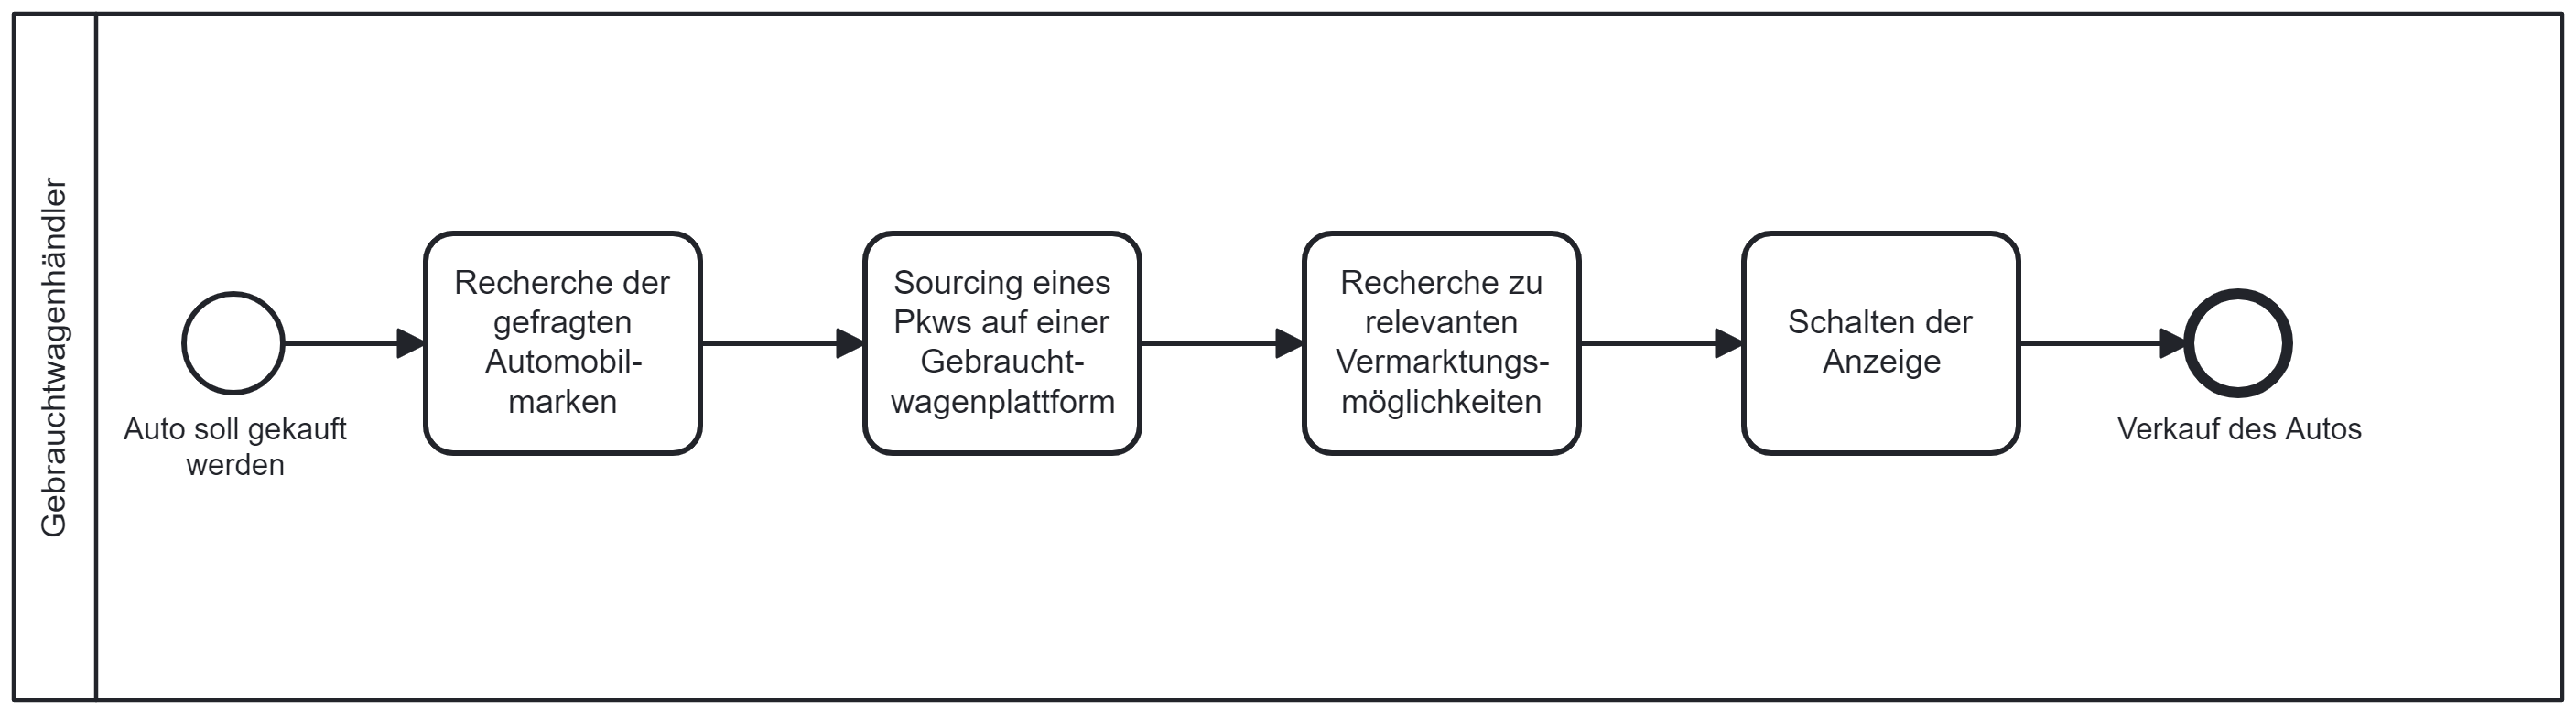
\includegraphics[width=\textwidth]{img/verkaufsprozess.png}
    \caption{Modellierung eines Geschäftsprozess eines Gebrauchtwagenhändlers mit Camunda Modeler}
    \label{fig:business-process}
\end{figure}
Anhand dieses Prozesses werden verschiedene Anwendungsfälle entwickelt, mit denen die Nützlichkeit der oben vorgestellten Visualisierungen erläutert werden soll: \\
\begin{itemize}
    \item Recherche einer relevanten Marke
    \item Recherche einer relevanten Anzeige
    \item Schalten einer optimierten Anzeige
\end{itemize}
\subsection{Starplot: Recherche einer relevanten Marke }

Um eine Vorauswahl zu tre
\subsection{Scatterplot: Recherche einer relevanten Anzeige }
\subsection{Parallelplot: Schalten einer optimierten Anzeige}


\section{Verwandte Arbeiten}

Um verwandte Arbeiten zu identifizieren wurde eine Literaturrecherche in der wissenschaftlichen Datenbank Google Scholar durchgeführt. \\
Dabei wurden die Keywords \glqq visual analysis\grqq, \glqq visualization\grqq , "\glqq offerings\grqq , \glqq used car\grqq  und \glqq online platform\grqq  verwendet und verschiedene wissenschaftliche Publikationen identifiziert. Zwei dieser Treffer sollen hier exemplarisch vorgestellt und Unterschiede und Gemeinsamkeiten der hier präsentierten Lösung identifiziert werden. \\

Das Forschungspapier \glqq  How much is my car worth? A methodology for predicting used cars prices using Random Forest \grqq \cite{pal2017much} präsentiert eine Methode zur Vorhersage von Gebrauchtwagenpreisen mithilfe von Random Forest. Die Autoren entwickeln ein Modell, das mithilfe von maschinellem Lernen den Preis von Gebrauchtwagen prognostiziert.\\
Für die Analyse des verwendeten Datensatzes, der von eBay-Kleinanzeigen stammt, nutzen die Autoren verschiedene Visualisierungen. Beispiele hierfür sind Bar-Charts, Boxplots und Scatterplots.  Einige der  Ergebnisse zeigen die Verteilung des Fahrzeugalters, den durchschnittlichen Preis nach Fahrzeugtyp, die Verteilung von Fahrzeugmarken und den Einfluss von reparierten Schäden auf den Fahrzeugpreis. \\

\begin{figure}[H]
    \centering
    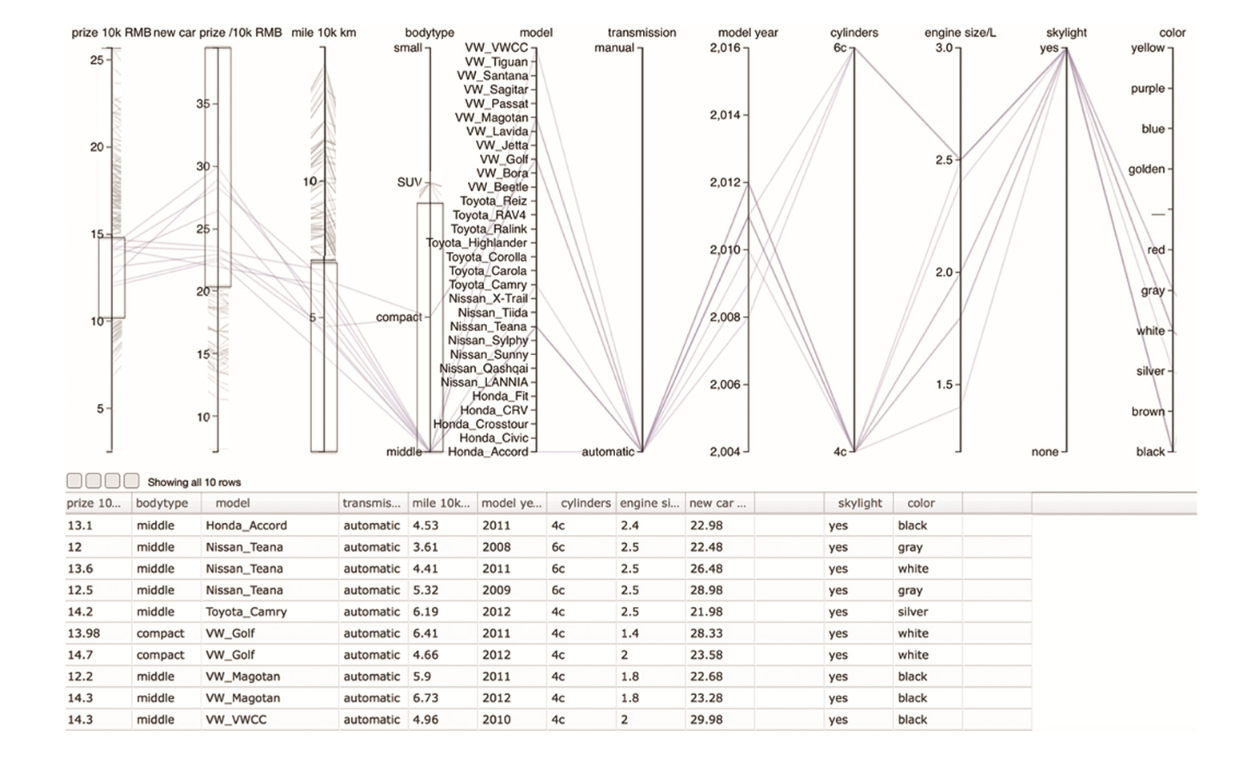
\includegraphics[width = \textwidth]{img/related_work.png}
    \caption{Vergleiche anderes Paper}
    \label{fig:related_work_vis}
\end{figure}

Die zweite Arbeit \cite{chen2017employing} beschäftigt sich mit der Verbesserung der Nutzerfahrung auf Gebrauchtwagen-Online-Plattformen mithilfe von Datenvisualisierungen. Die Autoren betonen die Komplexität der Daten und die Herausforderungen für Nutzer, zufriedenstellende Autos innerhalb ihres Budgets zu finden. \\

Sie analysieren das Verhalten von Autokäufern und entwickeln eine Datenvisualisierungsschnittstelle, wie sie auch im Kapitel zu Anwendungsfällen beschrieben ist. Die vorgestellte Parallelkoordinaten-Visualisierung ermöglicht es Benutzern, den Gebrauchtwagenmarkt zu verstehen, Beziehungen zwischen verschiedenen Attributen zu erkennen und Autos einfach zu suchen, filtern und vergleichen. Die Autoren identifizieren Probleme mit den aktuellen Suchmethoden, einschließlich Informationsüberlastung und -mangel, und stellen Designanforderungen vor. Die vorgeschlagene Schnittstelle ermöglicht es Benutzern, eine Übersicht des Marktes zu erhalten, Vorhersagen zu treffen, Kompromisse zwischen Attributen zu finden und eine geeignete Auswahl von Autos zu erstellen. Die Parallelkoordinaten-Plots werden auf der Suchseite implementiert, wobei verschiedene Parameter wie Preis, Typ, Kilometerstand, Baujahr und andere visuell dargestellt werden (Abbildung \ref{fig:related_work_vis}. Die Benutzer können mithilfe von Auswahlboxen auf den Achsen Suchbereiche festlegen und so eine engere Auswahl von Autos erstellen.\\
Insgesamt zeigt die Arbeit, wie Datenvisualisierung die Suche nach Gebrauchtwagen verbessern kann, indem sie dem Benutzer eine bessere Kontrolle, Vorhersagbarkeit und Verständnis des Marktes ermöglicht. \\


\section{Zusammenfassung und Ausblick}

Fassen sie die Beiträge ihre Visualisierungsanwendung zusammen. Wo bietet sie für die Personen der Zielgruppe einen echten Mehrwert.

Was wären mögliche sinnvolle Erweiterungen, entweder auf der Ebene der Visualisierungen und/oder auf der Datenebene?
\section*{Anhang: Git-Historie}

\clearpage
\pagenumbering{gobble}
\printbibliography[]

\end{document}

